%---------------------------------------------------------------------
\begin{frame}{What we have learned so far}

    \begin{enumerate}
        \item The U.S. healthcare system
        \begin{itemize}
            \item General facts
            \item Actors involved and how they relate
            \item Brief history of health insurance in the U.S.
        \end{itemize}
        \item How to think about the demand for health: the Grossman model (1972)
        \item Health insurance
        \begin{itemize}
            \item Demand for health insurance
            \begin{itemize}
                \item Why do people value health insurance?
                \item Understanding health insurance plans
            \end{itemize}
            \item Moral hazard: what does it mean for health insurance?
            \begin{itemize}
                \item What is the price elasticity of the demand for healthcare?
                \item What is the impact of health insurance on healthcare expenditures?
                \item Which type of care is cut?
                \item Ways to limit moral hazard? Coinsurance, deductible, prior authorization
            \end{itemize}
        \end{itemize}
    \end{enumerate}
    
\end{frame}
%---------------------------------------------------------------------
\begin{frame}{Next on our list}

    \begin{enumerate}
        \item[3.] Health insurance
        \begin{itemize}
            \item Demand for health insurance
            \item Moral hazard: what does it mean for health insurance?
            \item \textbf{Who \textit{select} into health insurance plans?} \newbold{Adverse selection}
        \end{itemize}
    \end{enumerate}
    
\end{frame}
%---------------------------------------------------------------------
\begin{frame}{Microeconomic review}

    The demand for a good is such that
    \begin{itemize}
        \item At $P=3,000$, $100$ consumers want to buy
        \item At $P=2,000$, $200$ consumers want to buy
        \item At $P=1,000$, $300$ consumers want to buy
    \end{itemize}

    $\implies$ What does the demand curve look like?

\end{frame}
%---------------------------------------------------------------------
\begin{frame}{Microeconomic review}

\begin{center}
    \begin{tikzpicture}[x=0.025cm, y=0.0020cm, scale=0.6] % makes y-axis visually longer

        % Axes
        \draw[->, thick] (0,0) -- (450,0) node[right] {$Q$};
        \draw[->, thick] (0,0) -- (0,4200) node[above] {$P$};
        
        % Ticks and labels
        \foreach \x in {100,200,300}
          \draw (\x,0) -- (\x,-120) node[below] {\x};
        
        \foreach \y in {1000,2000,3000}
          \draw (0,\y) -- (-12,\y) node[left] {\y};
        
        % Demand line from y-intercept to x-intercept: p = 4000 - 10Q
        %\draw[thick] (0,4000) -- (400,0);
        
        % Intercepts (optional)
        %\fill (0,4000) circle[radius=2pt] node[above left] {$(0,4000)$};
        %\fill (400,0) circle[radius=2pt] node[below right] {$(400,0)$};
        
        % Given points
        \fill (100,3000) circle[radius=2pt] node[above right] {};
        \fill (200,2000) circle[radius=2pt] node[above right] {};
        \fill (300,1000) circle[radius=2pt] node[above right] {};
        
    \end{tikzpicture}             
\end{center}
\end{frame}
%---------------------------------------------------------------------
\begin{frame}{Microeconomic review}

    \begin{center}
        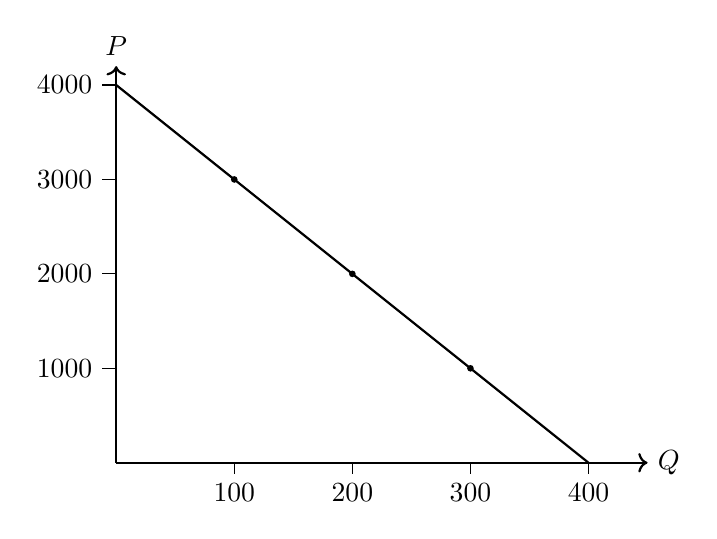
\begin{tikzpicture}[x=0.025cm, y=0.0020cm, scale=0.6] % makes y-axis visually longer
    
            % Axes
            \draw[->, thick] (0,0) -- (450,0) node[right] {$Q$};
            \draw[->, thick] (0,0) -- (0,4200) node[above] {$P$};
            
            % Ticks and labels
            \foreach \x in {100,200,300,400}
              \draw (\x,0) -- (\x,-120) node[below] {\x};
            
            \foreach \y in {1000,2000,3000,4000}
              \draw (0,\y) -- (-12,\y) node[left] {\y};
            
            % Demand line from y-intercept to x-intercept: p = 4000 - 10Q
            \draw[thick] (0,4000) -- (400,0);
            
            % Intercepts (optional)
            %\fill (0,4000) circle[radius=2pt] node[above left] {$(0,4000)$};
            %\fill (400,0) circle[radius=2pt] node[below right] {$(400,0)$};
            
            % Given points
            \fill (100,3000) circle[radius=2pt] node[above right] {};
            \fill (200,2000) circle[radius=2pt] node[above right] {};
            \fill (300,1000) circle[radius=2pt] node[above right] {};
            
        \end{tikzpicture}             
    \end{center}
    Demand: $P = 4,000 - 10Q$.

\end{frame}
%---------------------------------------------------------------------
\begin{frame}{Perfect competition}

    We have demand: $P = 4,000 - 10Q$.\\
    \vspace{5mm}
    The \newbold{marginal cost} is constant and equal to $1,500$\\
    \vspace{10mm}
    $\implies$ What is the price under \newbold{perfect competition}?
\end{frame}
%---------------------------------------------------------------------
\begin{frame}{Perfect competition}

    \newbold{Perfect competition}: firms are \textit{price takers}.
    \begin{align*}
        &\max_{Q} pQ-1,500Q\\
        \implies &P^{C} = 1,500\text{ }(p = \text{marginal cost})
    \end{align*}
    \vspace{2mm}
    We get quantities from the demand: $1,500 = 4,000 - 10 Q^{C} \implies Q^{C} = 250$\\
    \vspace{2mm}

    You can also get it using the \newbold{zero profit condition} $\pi = 0$:
    \begin{align*}
        \pi = 0 \implies &pQ - TC = 0\\
        &p = \frac{TC}{Q} \text{( =average cost)}\\
        &P^{C} = \frac{1,500 Q}{Q} = 1,500
    \end{align*}

\end{frame}
%---------------------------------------------------------------------
\begin{frame}{Perfect competition}

\begin{center}
    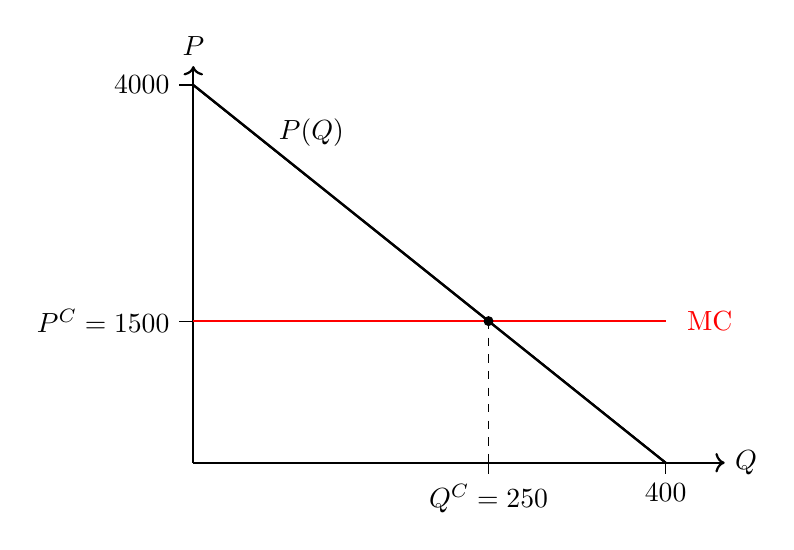
\begin{tikzpicture}[x=0.025cm, y=0.0020cm, scale=0.6]

        % Axes
        \draw[->, thick] (0,0) -- (450,0) node[right] {$Q$};
        \draw[->, thick] (0,0) -- (0,4200) node[above] {$P$};
        
        % Ticks and labels
        \foreach \x in {400}
          \draw (\x,0) -- (\x,-120) node[below] {\x};
        
        \foreach \y in {4000}
          \draw (0,\y) -- (-12,\y) node[left] {\y};

        \draw (0,1500) -- (-12,1500) node[left] {$P^{C}=1500$};
        \draw (250,0) -- (250,-120) node[below] {$Q^{C}=250$};

        % Demand line
        \draw[thick] (0,4000) -- (400,0);
        
        % Horizontal price line at p = 1500
        \draw[red, thick] (0,1500) -- (400,1500) node[right=4pt, red] {MC};
        
        % Intersection point
        \fill (250,1500) circle[radius=3pt];
        
        % Dashed projection lines
        \draw[dashed] (250,1500) -- (250,0);

        \draw[thick] (0,4000) -- (400,0);
        \node[above] at (100,3250) {$P(Q)$};        

    \end{tikzpicture}
\end{center}    
\end{frame}
%---------------------------------------------------------------------
\begin{frame}{Perfect competition + consumer surplus}

\begin{center}
    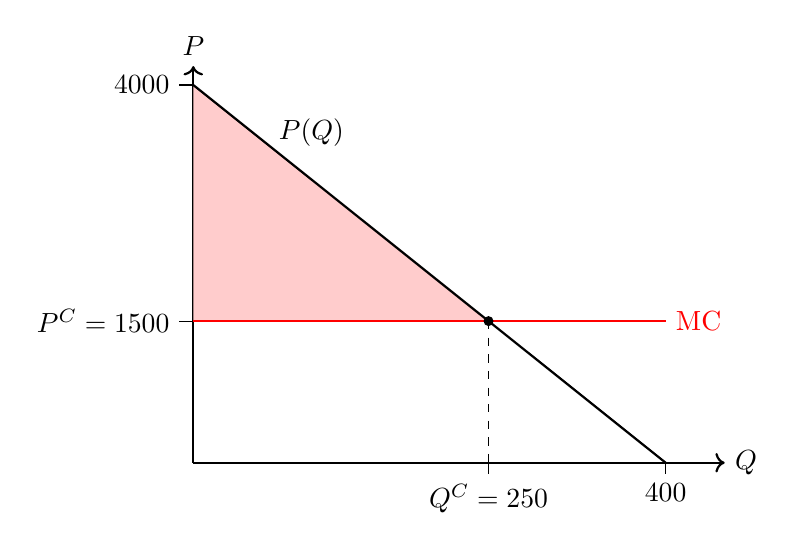
\begin{tikzpicture}[x=0.025cm, y=0.0020cm, scale=0.6]

        % Axes
        \draw[->, thick] (0,0) -- (450,0) node[right] {$Q$};
        \draw[->, thick] (0,0) -- (0,4200) node[above] {$P$};
        
        % X-axis ticks
        \foreach \x in {400}
            \draw (\x,0) -- (\x,-120) node[below] {\x};
        
        % Special x-axis tick at Q^{C}
        \draw (250,0) -- (250,-120) node[below] {$Q^{C}=250$};
        
        % Y-axis ticks
        \foreach \y in {4000}
            \draw (0,\y) -- (-12,\y) node[left] {\y};
        
        % Special y-axis tick at P^{C}
        \draw (0,1500) -- (-12,1500) node[left] {$P^{C}=1500$};
        
        % Shaded triangle (light red)
        \fill[red!20] (0,4000) -- (0,1500) -- (250,1500) -- cycle;
        
        % Demand curve
        \draw[thick] (0,4000) -- (400,0);
        \node[above] at (100,3250) {$P(Q)$};        
        
        % MC line
        \draw[red, thick] (0,1500) -- (400,1500)
            node[right, red] {MC};
        
        % Intersection point
        \fill (250,1500) circle[radius=3pt];
        
        % Dashed projection lines
        \draw[dashed] (250,1500) -- (250,0);

    
    \end{tikzpicture}    
\end{center}
\end{frame}
%---------------------------------------------------------------------
\begin{frame}{Monopoly}

    We have demand: $P = 4,000 - 10Q$.\\
    \vspace{5mm}
    The \newbold{marginal cost} is constant and equal to $1,500$\\
    \vspace{10mm}
    $\implies$ What is the price under \newbold{monopoly}?

\end{frame}
%---------------------------------------------------------------------
\begin{frame}{Monopoly}

    \newbold{Monopoly}: the firm \textit{chooses} the price, such that it maximizes profits.
    \begin{align*}
        \pi(Q) = P(Q)Q - 1,500Q
    \end{align*}

    We get
    \begin{align*}
        \max_{Q} \pi(Q) \implies &\frac{\partial \pi(Q)}{\partial Q} = 0\\
        &4,000 - 20 Q -1500 = 0\\
        & \underbrace{4,000 - 20 Q}_{\text{MR}} = \underbrace{1500}_{\text{MC}} \\
        & Q^{M} = 125
    \end{align*}
    and from the demand, we get $P^{M} = 2,750$.
    
\end{frame}
%---------------------------------------------------------------------
\begin{frame}{Monopoly}

    \begin{center}
        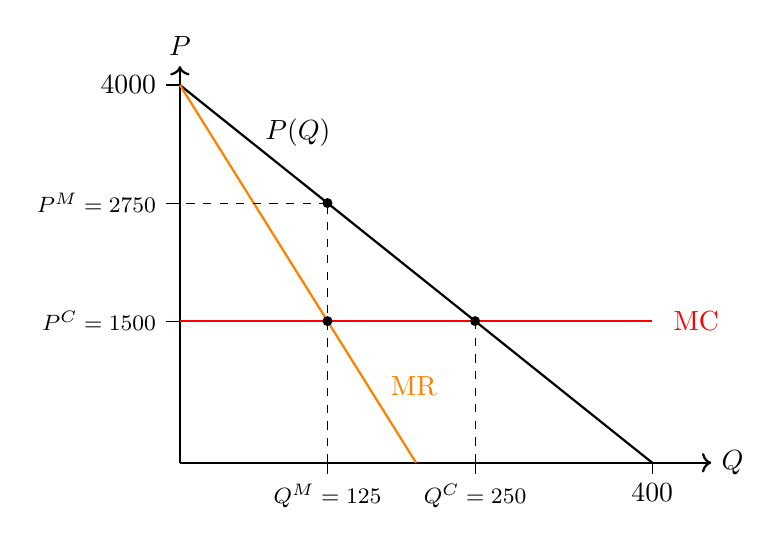
\begin{tikzpicture}[x=0.025cm, y=0.0020cm, scale=0.6]
        
            % Axes
            \draw[->, thick] (0,0) -- (450,0) node[right] {$Q$};
            \draw[->, thick] (0,0) -- (0,4200) node[above] {$P$};
            
            % Ticks and labels
            \foreach \x in {400}
                \draw (\x,0) -- (\x,-120) node[below] {\x};
            
            \foreach \y in {4000}
                \draw (0,\y) -- (-12,\y) node[left] {\y};
        
            % Special equilibrium labels
            \draw (0,1500) -- (-12,1500) node[left] {\footnotesize $P^{C}=1500$};
            \draw (250,0) -- (250,-120) node[below] {\footnotesize $Q^{C}=250$};
            \draw (0,2750) -- (-12,2750) node[left] {\footnotesize $P^{M}=2750$};
            \draw (125,0) -- (125,-120) node[below] {\footnotesize $Q^{M}=125$};

            % Demand curve P(Q)
            \draw[thick] (0,4000) -- (400,0);
            \node[above] at (100,3250) {$P(Q)$};
        
            % Marginal Cost
            \draw[red, thick] (0,1500) -- (400,1500) node[right=4pt, red] {MC};
            
            % Perfect competition intersection
            \fill (250,1500) circle[radius=3pt];
            \draw[dashed] (250,1500) -- (250,0);
        
            % New orange line: P = 4000 - 20Q
            \draw[orange, thick] (0,4000) -- (200,0)
                node[pos=0.85, above right, orange] {MR};
        
            % Monopoly intersection with MC at (125,1500)
            \fill (125,1500) circle[radius=3pt];
        
            % Correct dashed guides (as requested)
            \draw[dashed] (125,0) -- (125,2750);
            \draw[dashed] (125,2750) -- (0,2750);
        
            % Point on demand curve directly above monopoly quantity
            \fill (125,2750) circle[radius=3pt];
        
        \end{tikzpicture}
        \end{center}
            
\end{frame}
%---------------------------------------------------------------------
\begin{frame}{Monopoly + consumer surplus}

    \begin{center}
        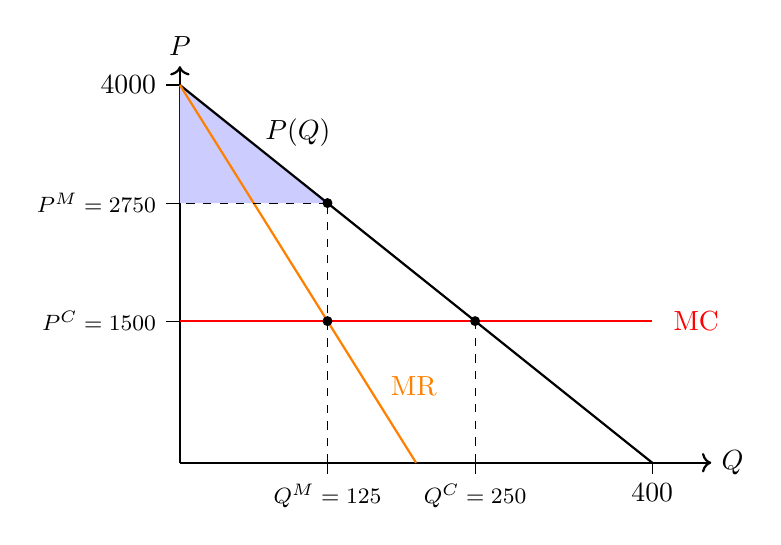
\begin{tikzpicture}[x=0.025cm, y=0.0020cm, scale=0.6]
        
            % Axes
            \draw[->, thick] (0,0) -- (450,0) node[right] {$Q$};
            \draw[->, thick] (0,0) -- (0,4200) node[above] {$P$};
            
            % Ticks and labels
            \foreach \x in {400}
                \draw (\x,0) -- (\x,-120) node[below] {\x};
            
            \foreach \y in {4000}
                \draw (0,\y) -- (-12,\y) node[left] {\y};
        
            % Special equilibrium labels
            \draw (0,1500) -- (-12,1500) node[left] {\footnotesize $P^{C}=1500$};
            \draw (250,0) -- (250,-120) node[below] {\footnotesize $Q^{C}=250$};
            \draw (0,2750) -- (-12,2750) node[left] {\footnotesize $P^{M}=2750$};
            \draw (125,0) -- (125,-120) node[below] {\footnotesize $Q^{M}=125$};
        
            % Monopoly consumer surplus (light blue)
            \fill[blue!20] (0,4000) -- (0,2750) -- (125,2750) -- cycle;
        
            % Demand curve
            \draw[thick] (0,4000) -- (400,0);
            \node[above] at (100,3250) {$P(Q)$};
        
            % Marginal Cost
            \draw[red, thick] (0,1500) -- (400,1500) node[right=4pt, red] {MC};
            
            % Perfect competition intersection
            \fill (250,1500) circle[radius=3pt];
            \draw[dashed] (250,1500) -- (250,0);
        
            % Marginal Revenue
            \draw[orange, thick] (0,4000) -- (200,0)
                node[pos=0.85, above right, orange] {MR};
        
            % Monopoly intersection with MC
            \fill (125,1500) circle[radius=3pt];
        
            % Monopoly guides
            \draw[dashed] (125,0) -- (125,2750);
            \draw[dashed] (125,2750) -- (0,2750);
        
            % Monopoly price point on demand
            \fill (125,2750) circle[radius=3pt];
        
        \end{tikzpicture}
        \end{center}
            
\end{frame}
%---------------------------------------------------------------------
\begin{frame}{Asymmetric information}

    \newbold{Asymmetric information} arises when one side of the market
    (i.e., the buyers or the sellers) have \textbf{information} that the other side does not have\\
    $\implies$ The ``Akerlof lemons problem'' refers to the situation where used car sellers
    have information on the quality of a used car, which buyers cannot observe
    (i.e., sellers have a “hidden type”)

    \vspace{3mm}
    \only<1>{
        \vspace{15mm}

    }
    \only<2>{$\implies$ Do we have asymmetric information in health insurance?
    
    \vspace{10mm}}

    \only<3>{$\implies$ Do we have asymmetric information in health insurance?
    {\color{blue} Buyers of insurance may have more information about their health than insurers.}}
    
    
\end{frame}
%---------------------------------------------------------------------
\begin{frame}{Selection markets}

    Markets where the identity of the consumer who buys determines both willingness to pay for the product and production costs 
    are called \newbold{selection markets} (e.g., health insurance, consumer credit markets, mortgage markets, ...)\\
    $\implies$ The seller does not only cares about how much they sell but \textit{to whom they sell too}.
    \vspace{3mm}

    Asymmetric information: the producer cannot exactly tell who each consumer is\\
    \textit{Health insurance}: sicker consumers buy insurance first $\implies$ \newbold{adverse selection}
    \vspace{3mm}

    What strategies can firms develop to fight adverse selection?
    \begin{itemize}
        \item Insurance rejections (e.g. refuse to cover people with pre-existing conditions)
        \item Cream-skimming: use of a contract feature as a screening device (e.g. do not reimburse drugs used by sicker patients)
    \end{itemize}
    
\end{frame}
%---------------------------------------------------------------------
\begin{frame}{Adverse selection}

    \newbold{Adverse selection} in health insurance:
    individuals buying insurance have worse health and/or higher expected costs than the individuals who choose to remain uninsured.\\
    It can be 
    \begin{itemize}
        \item Between being insured/uninsured
        \item Between different insurance plans
    \end{itemize}
    \vspace{5mm}

    Adverse selection is one of the textbook rationales for \newbold{government involvement} in health insurance markets.
    \begin{itemize}
        \item Absent government intervention, the insurance market will be inefficient and ``adversely selected''
    $\implies$ \newbold{Market failure}
    \end{itemize}
    
\end{frame}
%---------------------------------------------------------------------
\begin{frame}{}

    \begin{center}
        \Large \textcolor{maroon}{Let's see what it looks like in our microeconomic framework}
    \end{center}
\end{frame}
%---------------------------------------------------------------------
\begin{frame}{Setup}

    In the next slides, we will care only about the price of 
    the insurance contract (premium) and \textbf{ignore/fix the rest of 
    the contract features} (e.g. deductible, coinsurance, ...)\\
     $\implies$
    \textit{We are thinking about the demand for one specific insurance contract with only the premium varying}\\
    \vspace{5mm}

    New demand:
    \begin{itemize}
        \item At $P=4,000$, 92 consumers want to buy
        \item At $P=2,000$, 246 consumers want to buy
        \item At $P=1,000$, 323 consumers want to buy
    \end{itemize}

\end{frame}
%---------------------------------------------------------------------
\begin{frame}{Demand}

    \begin{center}
    \begin{tikzpicture}[x=0.035cm, y=0.0020cm, scale=0.55]

        % Axes (longer x-axis)
        \draw[->, thick] (0,0) -- (520,0) node[right] {$Q$};
        \draw[->, thick] (0,0) -- (0,5600) node[above] {$P$};

        % Demand line
        \draw[thick] (0,5200) -- (400,0);

        % Intercepts with labels
        \fill (0,5200) circle[radius=3pt];
        \node[left] at (0,5200) {};

        \fill (400,0) circle[radius=3pt];
        \node[below] at (400,0) {};

        % Given points with axis projections and labels
        
        % Point 1
        \fill (92,4000) circle[radius=3pt];
        \draw[dashed] (92,0) -- (92,4000);
        \draw[dashed] (0,4000) -- (92,4000);
        \node[below] at (92,0) {$92$};
        \node[left] at (0,4000) {$4000$};

        % Point 2
        \fill (246,2000) circle[radius=3pt];
        \draw[dashed] (246,0) -- (246,2000);
        \draw[dashed] (0,2000) -- (246,2000);
        \node[below] at (246,0) {$246$};
        \node[left] at (0,2000) {$2000$};

        % Point 3
        \fill (323,1000) circle[radius=3pt];
        \draw[dashed] (323,0) -- (323,1000);
        \draw[dashed] (0,1000) -- (323,1000);
        \node[below] at (323,0) {$323$};
        \node[left] at (0,1000) {$1000$};

    \end{tikzpicture}
\end{center}
\end{frame}
%---------------------------------------------------------------------
\begin{frame}{Setup}

    New demand:
    \begin{itemize}
        \item At $P=4,000$, 92 consumers want to buy
        \item At $P=2,000$, 246 consumers want to buy
        \item At $P=1,000$, 323 consumers want to buy
    \end{itemize}

    $\implies$ What does the demand curve look like? \only<1>{Solve for $a$ and $b$ such that}\only<2>{{\color{red} $P = 5,200 - 13Q$}}
    \[
    \begin{cases}
    4,000 = a + 92b \\
    2,000 = a + 246b
    \end{cases}
    \implies a \approx 5,200 \text{ and }b \approx -13
    \]
    
\end{frame}
%---------------------------------------------------------------------
\begin{frame}{Demand}

    \begin{center}
    \begin{tikzpicture}[x=0.035cm, y=0.0020cm, scale=0.55]

        % Axes (longer x-axis)
        \draw[->, thick] (0,0) -- (520,0) node[right] {$Q$};
        \draw[->, thick] (0,0) -- (0,5600) node[above] {$P$};

        % Demand line
        \draw[thick] (0,5200) -- (400,0);

        % Intercepts with labels
        \fill (0,5200) circle[radius=3pt];
        \node[left] at (0,5200) {$5200$};

        \fill (400,0) circle[radius=3pt];
        \node[below] at (400,0) {$400$};

        % Given points with axis projections and labels
        
        % Point 1
        \fill (92,4000) circle[radius=3pt];
        \draw[dashed] (92,0) -- (92,4000);
        \draw[dashed] (0,4000) -- (92,4000);
        \node[below] at (92,0) {$92$};
        \node[left] at (0,4000) {$4000$};

        % Point 2
        \fill (246,2000) circle[radius=3pt];
        \draw[dashed] (246,0) -- (246,2000);
        \draw[dashed] (0,2000) -- (246,2000);
        \node[below] at (246,0) {$246$};
        \node[left] at (0,2000) {$2000$};

        % Point 3
        \fill (323,1000) circle[radius=3pt];
        \draw[dashed] (323,0) -- (323,1000);
        \draw[dashed] (0,1000) -- (323,1000);
        \node[below] at (323,0) {$323$};
        \node[left] at (0,1000) {$1000$};

    \end{tikzpicture}
\end{center}
\end{frame}
%---------------------------------------------------------------------
\begin{frame}{Adding the cost}

    New demand:
    \begin{itemize}
        \item At $P=4,000$, 92 consumers want to buy\\
        {\color{blue} The expected healthcare cost for the 92nd individual is 3,080}
        \item At $P=2,000$, 246 consumers want to buy\\
        {\color{blue} The expected healthcare cost for the 246th individual is 1,540}
        \item At $P=1,000$, 323 consumers want to buy\\
        {\color{blue} The expected healthcare cost for the 323rd individual is 770}
    \end{itemize}

    $\implies$ What is the \newbold{marginal cost}?

\end{frame}
%---------------------------------------------------------------------
\begin{frame}{Demand and marginal cost}

    \begin{center}
    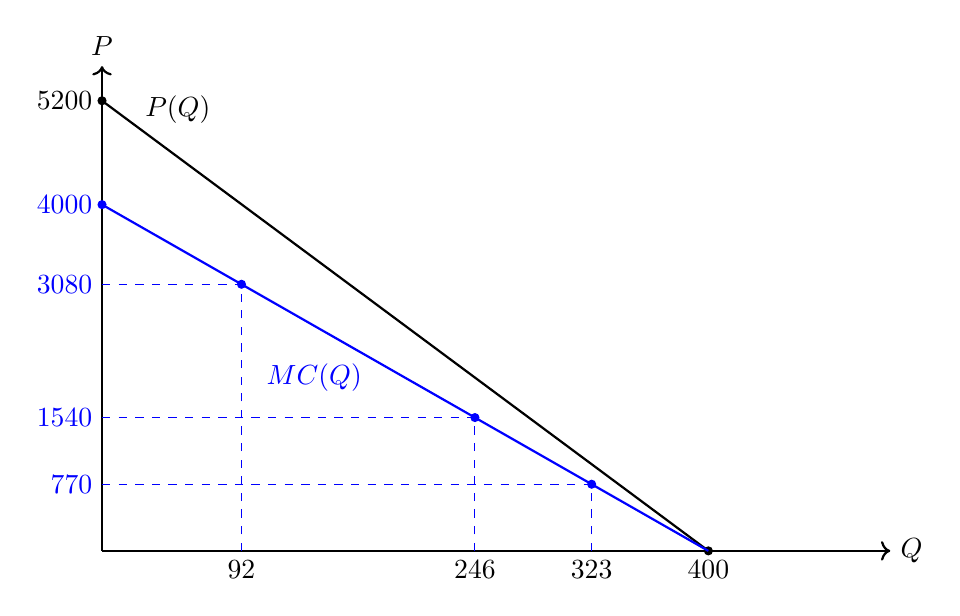
\begin{tikzpicture}[x=0.035cm, y=0.0020cm, scale=0.55]

        % Axes
        \draw[->, thick] (0,0) -- (520,0) node[right] {$Q$};
        \draw[->, thick] (0,0) -- (0,5600) node[above] {$P$};

        % Demand curve
        \draw[thick] (0,5200) -- (400,0);
        \node at (50,5100) {$P(Q)$};

        % Demand intercepts
        \fill (0,5200) circle[radius=3pt];
        \node[left] at (0,5200) {$5200$};

        \fill (400,0) circle[radius=3pt];
        \node[below] at (400,0) {$400$};

        % Expected cost curve
        \draw[blue, thick] (0,4000) -- (400,0);
        \node[blue] at (140,2005) {$MC(Q)$};

        % Expected cost intercept
        \fill[blue] (0,4000) circle[radius=3pt];
        \node[left, blue] at (0,4000) {$4000$};

        % Expected cost points and projections

        % Point 1
        \fill[blue] (92,3080) circle[radius=3pt];
        \draw[dashed, blue] (92,0) -- (92,3080);
        \draw[dashed, blue] (0,3080) -- (92,3080);
        \node[below] at (92,0) {$92$};
        \node[left, blue] at (0,3080) {$3080$};

        % Point 2
        \fill[blue] (246,1540) circle[radius=3pt];
        \draw[dashed, blue] (246,0) -- (246,1540);
        \draw[dashed, blue] (0,1540) -- (246,1540);
        \node[below] at (246,0) {$246$};
        \node[left, blue] at (0,1540) {$1540$};

        % Point 3
        \fill[blue] (323,770) circle[radius=3pt];
        \draw[dashed, blue] (323,0) -- (323,770);
        \draw[dashed, blue] (0,770) -- (323,770);
        \node[below] at (323,0) {$323$};
        \node[left, blue] at (0,770) {$770$};

    \end{tikzpicture}
    \end{center}
\end{frame}
%---------------------------------------------------------------------
\begin{frame}{Demand, marginal cost}

    New demand:
    \begin{itemize}
        \item At $P=4,000$, 92 consumers want to buy\\
        {\color{blue} The expected healthcare cost for the 92nd individual is 3,080}
        \item At $P=2,000$, 246 consumers want to buy\\
        {\color{blue} The expected healthcare cost for the 246th individual is 1,540}
        \item At $P=1,000$, 323 consumers want to buy\\
        {\color{blue} The expected healthcare cost for the 323rd individual is 770}
    \end{itemize}
    $\implies$ Demand: $P = 5,200 - 13Q$\\
    $\implies$ Marginal cost (MC): $4,000 - 10Q$\\
    \vspace{2mm}
    Note: the demand and marginal cost \newbold{are tied together!}
\end{frame}
%---------------------------------------------------------------------
\begin{frame}{Demand, marginal cost, and risk premium}

    Risk premium (RP): $ P(Q) = \underbrace{MC(Q)}_{\text{expected cost}} + {\color{red} RP} \implies {\color{red} RP} = P(Q) - MC(Q)$

    \begin{center}
    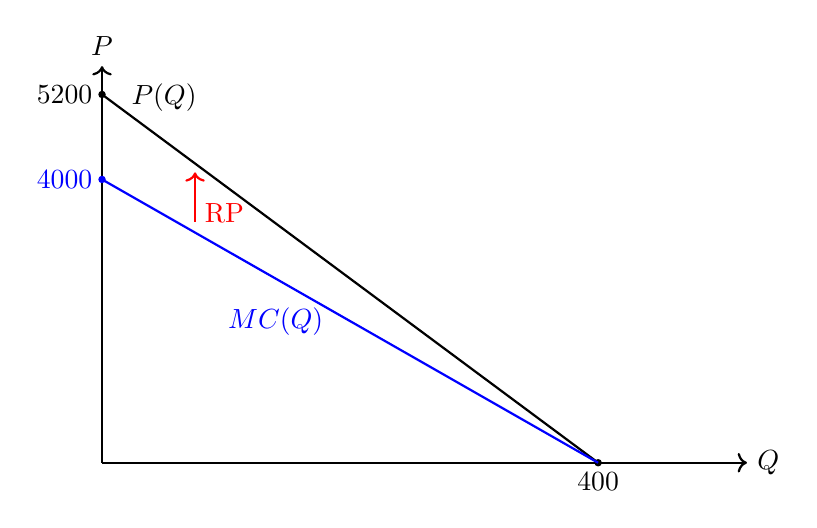
\begin{tikzpicture}[x=0.035cm, y=0.0020cm, scale=0.45]

        % Axes
        \draw[->, thick] (0,0) -- (520,0) node[right] {$Q$};
        \draw[->, thick] (0,0) -- (0,5600) node[above] {$P$};

        % Demand curve
        \draw[thick] (0,5200) -- (400,0);
        \node at (50,5150) {$P(Q)$};

        % Demand intercepts
        \fill (0,5200) circle[radius=3pt];
        \node[left] at (0,5200) {$5200$};

        \fill (400,0) circle[radius=3pt];
        \node[below] at (400,0) {$400$};

        % Expected cost curve
        \draw[blue, thick] (0,4000) -- (400,0);
        \node[blue] at (140,1995) {$MC(Q)$};

        % Expected cost intercept
        \fill[blue] (0,4000) circle[radius=3pt];
        \node[left, blue] at (0,4000) {$4000$};

        % Red arrow showing risk premium
        \draw[red, thick, ->] (75,3400) -- (75,4100);
        \node[red, right] at (75,3525) {RP};

    \end{tikzpicture}
    \end{center}
\end{frame}
%---------------------------------------------------------------------
\begin{frame}{Demand, marginal cost, and \newbold{average cost}}

    New demand:
    \begin{itemize}
        \item At $P=4,000$, 92 consumers want to buy\\
        {\color{blue} The expected healthcare cost for the 92nd individual is 3,080}
        \item At $P=2,000$, 246 consumers want to buy\\
        {\color{blue} The expected healthcare cost for the 246th individual is 1,540}
        \item At $P=1,000$, 323 consumers want to buy\\
        {\color{blue} The expected healthcare cost for the 323rd individual is 770}
    \end{itemize}
    $\implies$ Demand: $P = 5,200 - 13Q$\\
    $\implies$ Marginal cost (MC): $MC = 4,000 - 10Q$\\
    $\implies$ What is the \newbold{average cost}?
\end{frame}
%---------------------------------------------------------------------
\begin{frame}{Demand, marginal cost, and \newbold{average cost}}

    Average cost ($AC(Q)$):
    \begin{align*}
        AC(Q) = \frac{TC(Q)}{Q}
    \end{align*}

    What is the total cost ($TC(Q)$)?
    \begin{align*}
        TC(Q) &= \int_0^Q MC(Q) dQ\\
        &= \int_0^Q (4000 - 10Q) dQ\\
        %&= [4,000Q - 5Q^2]_0^Q\\
        &= 4,000 Q - 5 Q^2
    \end{align*}

    We get
    \begin{align*}
        AC(Q) = \frac{TC(Q)}{Q} = 4,000 - 5 Q
    \end{align*}

\end{frame}
%---------------------------------------------------------------------
\begin{frame}{Demand, marginal cost, and average cost}

\begin{center}
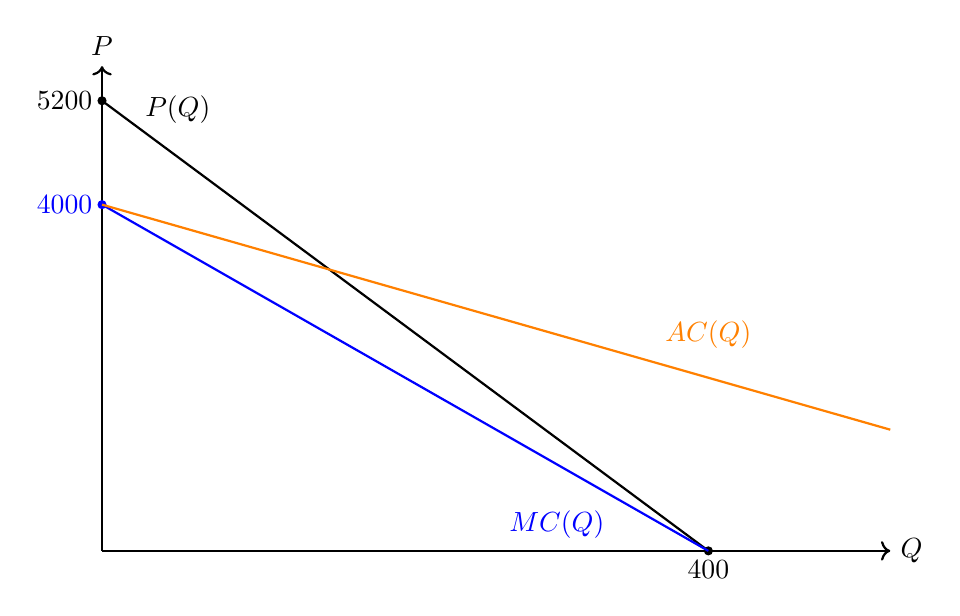
\begin{tikzpicture}[x=0.035cm, y=0.0020cm, scale=0.55]

    % Axes
    \draw[->, thick] (0,0) -- (520,0) node[right] {$Q$};
    \draw[->, thick] (0,0) -- (0,5600) node[above] {$P$};

    % Demand curve: P(Q) = 5200 - 13Q
    \draw[thick] (0,5200) -- (400,0);
    \node at (50,5100) {$P(Q)$};

    % Demand intercepts
    \fill (0,5200) circle[radius=3pt];
    \node[left] at (0,5200) {$5200$};

    \fill (400,0) circle[radius=3pt];
    \node[below] at (400,0) {$400$};

    % Marginal cost curve: MC(Q) = 4000 - 10Q
    \draw[blue, thick] (0,4000) -- (400,0);
    \node[blue] at (300,300) {$MC(Q)$};

    % MC intercept
    \fill[blue] (0,4000) circle[radius=3pt];
    \node[left, blue] at (0,4000) {$4000$};

    % Average cost curve: AC(Q) = 4000 - 5Q
    \draw[orange, thick] (0,4000) -- (520,1400);
    \node[orange] at (400,2500) {$AC(Q)$};

\end{tikzpicture}
\end{center}
\end{frame}
%---------------------------------------------------------------------
\begin{frame}{Demand, marginal cost, and average cost}

    New demand:
    \begin{itemize}
        \item At $P=4,000$, 92 consumers want to buy\\
        {\color{blue} The expected healthcare cost for the 92nd individual is 3,080}
        \item At $P=2,000$, 246 consumers want to buy\\
        {\color{blue} The expected healthcare cost for the 246th individual is 1,540}
        \item At $P=1,000$, 323 consumers want to buy\\
        {\color{blue} The expected healthcare cost for the 323rd individual is 770}
    \end{itemize}
    $\implies$ Demand: $P(Q) = 5,200 - 13Q$\\
    $\implies$ Marginal cost (MC): $MC(Q) = 4,000 - 10Q$\\
    $\implies$ Average cost (AC): $AC(Q) = 4,000 - 5 Q$\\
    \vspace{3mm}

    $\implies$ What si the \newbold{efficient} allocation?

\end{frame}
%---------------------------------------------------------------------
\begin{frame}{Efficient allocation}

    Efficient allocation: $P(Q)=MC(Q)$
    \begin{align*}
        P(Q) = 4,000 - 10 Q\\
        5,200 - 13Q = 4,000 - 10 Q\\
        1,200 = 3Q\\
        Q^{EFF}= 400
    \end{align*}
    and $P^{EFF} = 5,200 - 13 \times 400 = 0$.\\
    \vspace{5mm}
    $\implies$ Full insurance is efficient here:
    all consumers buy insurance, since their marginal cost
    is below their demand (all have a risk premium $\geq 0$).
\end{frame}
%---------------------------------------------------------------------
\begin{frame}{Efficient equilibrium}

\begin{center}
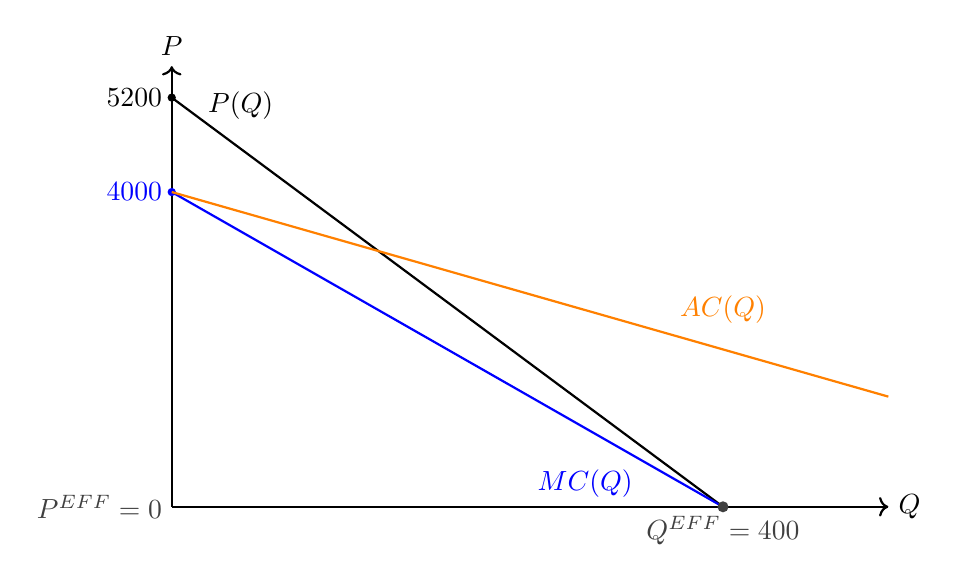
\begin{tikzpicture}[x=0.035cm, y=0.0020cm, scale=0.5]

    % Axes
    \draw[->, thick] (0,0) -- (520,0) node[right] {$Q$};
    \draw[->, thick] (0,0) -- (0,5600) node[above] {$P$};

    % Demand curve: P(Q) = 5200 - 13Q
    \draw[thick] (0,5200) -- (400,0);
    \node at (50,5100) {$P(Q)$};

    % Demand intercepts
    \fill (0,5200) circle[radius=3pt];
    \node[left] at (0,5200) {$5200$};

    \fill (400,0) circle[radius=3pt];
    \node[below] at (400,0) {};

    % Marginal cost curve: MC(Q) = 4000 - 10Q
    \draw[blue, thick] (0,4000) -- (400,0);
    \node[blue] at (300,300) {$MC(Q)$};

    \fill[blue] (0,4000) circle[radius=3pt];
    \node[left, blue] at (0,4000) {$4000$};

    % Average cost curve: AC(Q) = 4000 - 5Q
    \draw[orange, thick] (0,4000) -- (520,1400);
    \node[orange] at (400,2500) {$AC(Q)$};

    % Efficient equilibrium (dark gray)
    \fill[darkgray] (400,0) circle[radius=4pt];
    \node[below, darkgray] at (400,0) {$Q^{EFF}=400$};
    \node[left, darkgray] at (0,0) {$P^{EFF}=0$};

\end{tikzpicture}
\end{center} 
\end{frame}
%---------------------------------------------------------------------
\begin{frame}{Efficient allocation}

    Efficient allocation: $Q^{EFF}= 400$ and $P^{EFF} = 0$\\
    \vspace{5mm}

    Note however that at this price:
    \begin{align*}
        \pi(P^{EFF}) &= 0 - 800,000\\
        &<0
    \end{align*}
    $\implies$ No firms would offer this price! Why?\\
    \pause
    Because the price is below the average cost!\\
    \pause
    \vspace{3mm}
    $\implies$ What will the \newbold{competitive equilibrium} be?

\end{frame}
%---------------------------------------------------------------------
\begin{frame}{Efficient and perfect competition equilibria}

    The perfect competition equilibrium will be at $\pi(Q) = 0$:
    \begin{align*}
        p(Q)Q - TC(Q) &= 0\\
        p(Q) = AC(Q)\\
        5,200 - 13Q = 4,000 - 5 Q\\
        Q^{C} = 150
    \end{align*}
    and we get $P^{C} = 3,250$.

\end{frame}
%---------------------------------------------------------------------
\begin{frame}{Efficient and perfect competition equilibria}

\begin{center}
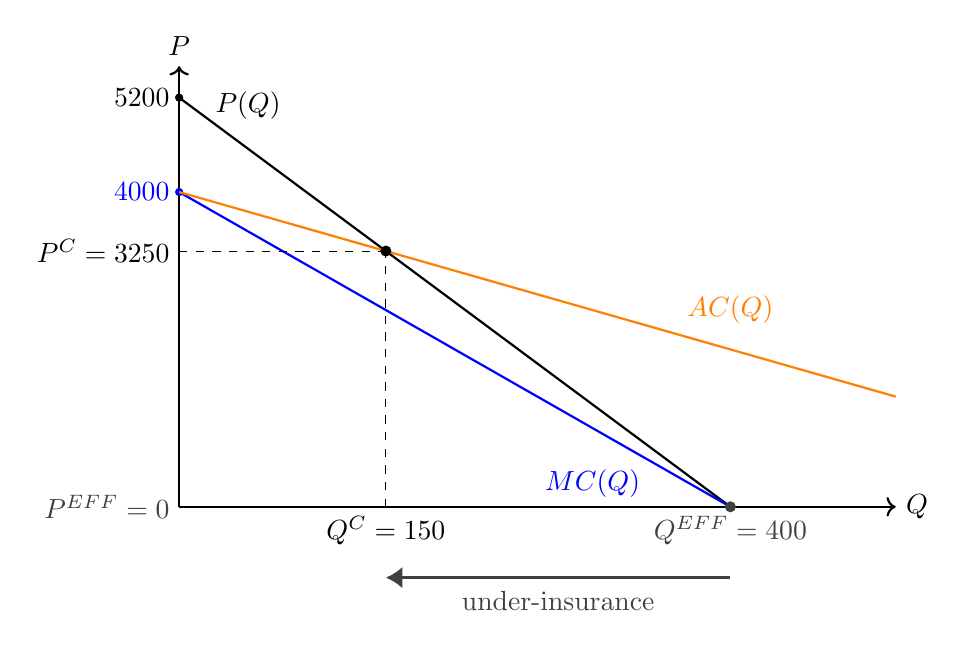
\begin{tikzpicture}[x=0.035cm, y=0.0020cm, scale=0.5]

    % Axes
    \draw[->, thick] (0,0) -- (520,0) node[right] {$Q$};
    \draw[->, thick] (0,0) -- (0,5600) node[above] {$P$};

    % Demand curve: P(Q) = 5200 - 13Q
    \draw[thick] (0,5200) -- (400,0);
    \node at (50,5100) {$P(Q)$};

    % Demand intercepts
    \fill (0,5200) circle[radius=3pt];
    \node[left] at (0,5200) {$5200$};

    \fill (400,0) circle[radius=3pt];
    \node[below] at (400,0) {};

    % Marginal cost curve: MC(Q) = 4000 - 10Q
    \draw[blue, thick] (0,4000) -- (400,0);
    \node[blue] at (300,300) {$MC(Q)$};

    \fill[blue] (0,4000) circle[radius=3pt];
    \node[left, blue] at (0,4000) {$4000$};

    % Average cost curve: AC(Q) = 4000 - 5Q
    \draw[orange, thick] (0,4000) -- (520,1400);
    \node[orange] at (400,2500) {$AC(Q)$};

    % Perfect competition equilibrium (black)
    \fill (150,3250) circle[radius=4pt];
    \draw[dashed] (150,0) -- (150,3250);
    \draw[dashed] (0,3250) -- (150,3250);

    \node[below] at (150,0) {$Q^{C}=150$};
    \node[left] at (0,3250) {$P^{C}=3250$};

    % Efficient equilibrium (dark gray)
    \fill[darkgray] (400,0) circle[radius=4pt];
    \node[below, darkgray] at (400,0) {$Q^{EFF}=400$};
    \node[left, darkgray] at (0,0) {$P^{EFF}=0$};

    % Under-insurance arrow under x-axis (EFF -> PC), arrowhead on the left
    \draw[-{Latex[length=6pt,width=8pt]}, very thick, darkgray] (400,-900) -- (150,-900);
    \node[darkgray] at (275,-1200) {under-insurance};

\end{tikzpicture}
\end{center} 
\end{frame}
%---------------------------------------------------------------------
\begin{frame}{Demand, marginal cost, and average cost}

    New demand:
    \begin{itemize}
        \item At $P=4,000$, 92 consumers want to buy\\
        {\color{blue} The expected healthcare cost for the 92nd individual is 3,080}
        \item At $P=2,000$, 246 consumers want to buy\\
        {\color{blue} The expected healthcare cost for the 246th individual is 1,540}
        \item At $P=1,000$, 323 consumers want to buy\\
        {\color{blue} The expected healthcare cost for the 323rd individual is 770}
    \end{itemize}
    $\implies$ Demand: $P = 5,200 - 13Q$\\
    $\implies$ Marginal cost (MC): $MC = 4,000 - 10Q$\\
    $\implies$ Average cost (AC): $AC = 4,000 - 5 Q$\\
    \vspace{3mm}

    $\implies$ What if we had a \newbold{monopolist}?

\end{frame}
%---------------------------------------------------------------------
\begin{frame}{Monopoly}

    The \newbold{monopolist} would choose prices to maximize profits:
    \begin{align*}
        &\max_Q \pi(Q) = p(Q)Q - AC(Q)Q = 5,200Q - 13Q^2 - 4,000Q - 5Q^2\\
        \implies &\frac{\partial \pi(Q)}{\partial Q} = 0\\
        &\underbrace{5,200 - 26Q}_{MR(Q)} - \underbrace{4,000 - 10 Q}_{MC(Q)} = 0\\
        &Q^{M} = 75
    \end{align*}
    and we get $P^{M} = 4,225$.\\

\end{frame}
%---------------------------------------------------------------------
\begin{frame}{Monopoly}

\begin{center}
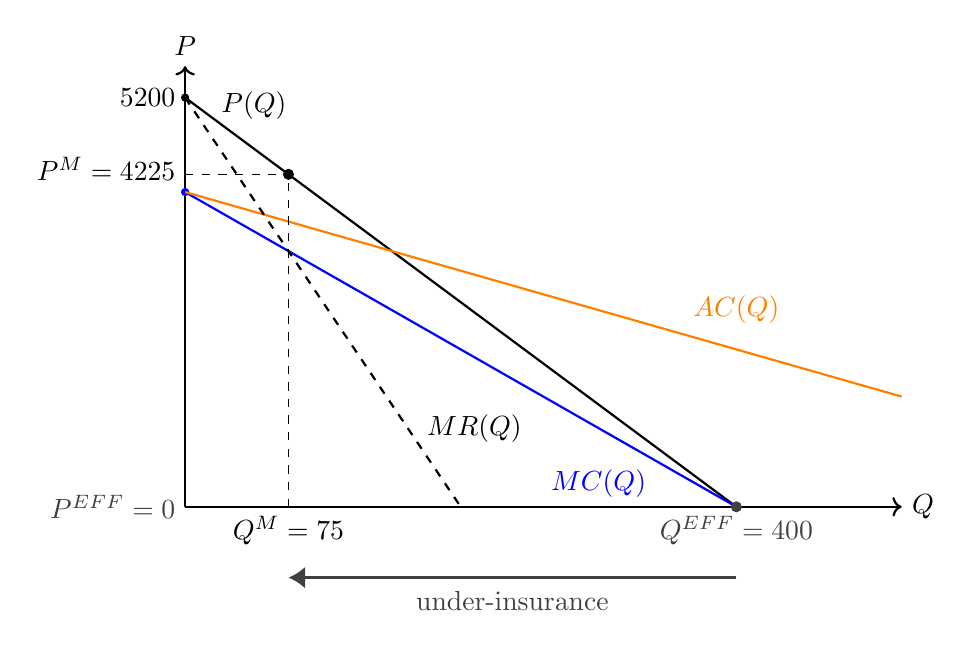
\begin{tikzpicture}[x=0.035cm, y=0.0020cm, scale=0.5]

    % Axes
    \draw[->, thick] (0,0) -- (520,0) node[right] {$Q$};
    \draw[->, thick] (0,0) -- (0,5600) node[above] {$P$};

    % Demand curve: P(Q) = 5200 - 13Q
    \draw[thick] (0,5200) -- (400,0);
    \node at (50,5100) {$P(Q)$};

    % Demand intercepts
    \fill (0,5200) circle[radius=3pt];
    \node[left] at (0,5200) {$5200$};

    \fill (400,0) circle[radius=3pt];
    \node[below] at (400,0) {};

    % Marginal cost curve: MC(Q) = 4000 - 10Q
    \draw[blue, thick] (0,4000) -- (400,0);
    \node[blue] at (300,300) {$MC(Q)$};

    \fill[blue] (0,4000) circle[radius=3pt];
    \node[left, blue] at (0,4000) {};

    % Average cost curve: AC(Q) = 4000 - 5Q
    \draw[orange, thick] (0,4000) -- (520,1400);
    \node[orange] at (400,2500) {$AC(Q)$};

    % MR curve: twice the slope of demand (dashed black)
    % Demand slope is -13, so MR slope is -26 with same intercept 5200:
    % MR(Q) = 5200 - 26Q
    \draw[dashed, thick] (0,5200) -- (200,0);
    \node at (210,1000) {$MR(Q)$};

    % Monopolist equilibrium: intersection of MR and MC (given)
    \fill (75,4225) circle[radius=4pt];
    \draw[dashed] (75,0) -- (75,4225);
    \draw[dashed] (0,4225) -- (75,4225);

    \node[below] at (75,0) {$Q^{M}=75$};
    \node[left] at (0,4300) {$P^{M}=4225$};

    % Efficient equilibrium (dark gray)
    \fill[darkgray] (400,0) circle[radius=4pt];
    \node[below, darkgray] at (400,0) {$Q^{EFF}=400$};
    \node[left, darkgray] at (0,0) {$P^{EFF}=0$};

    % Under-insurance arrow under x-axis (EFF -> MONOP), arrowhead on the left
    \draw[-{Latex[length=6pt,width=8pt]}, very thick, darkgray] (400,-900) -- (75,-900);
    \node[darkgray] at (237.5,-1200) {under-insurance};

\end{tikzpicture}
\end{center}
\end{frame}
%---------------------------------------------------------------------
\begin{frame}{Adverse selection}

    \newbold{Adverse selection} in health insurance:
    individuals buying insurance have worse health and/or higher expected costs than the individuals who choose to remain uninsured.\\
    $\implies$ The cost and demand curves \newbold{depend on each other}: \textit{selection market}
    $\implies$ \textit{Adverse selection}: the cost curves \newbold{slope down}\\
    \vspace{5mm}
    \textit{Note: the exact equilibria, amount of under-insurance, etc. depend on the demand and cost curves we assumed.}\\
    \vspace{5mm}

    Could the market completely unravel? \only<2>{\newbold{yes...}}
\end{frame}
%---------------------------------------------------------------------
\begin{frame}{Adverse selection}

\begin{center}
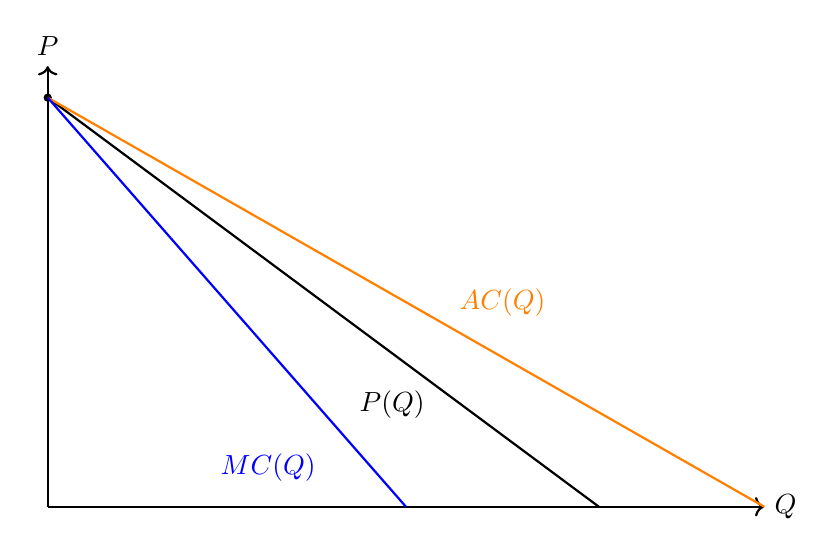
\begin{tikzpicture}[x=0.035cm, y=0.0020cm, scale=0.5]

    % Axes
    \draw[->, thick] (0,0) -- (520,0) node[right] {$Q$};
    \draw[->, thick] (0,0) -- (0,5600) node[above] {$P$};

    % Common intercept
    \fill (0,5200) circle[radius=3pt];
    \node[left] at (0,5200) {};

    % Demand curve: P(Q) = 5200 - 13Q
    \draw[thick] (0,5200) -- (400,0);
    \node at (250,1300) {$P(Q)$};

    % Average cost curve above demand: AC(Q) = 5200 - 10Q  (flatter)
    \draw[orange, thick] (0,5200) -- (520,0);
    \node[orange] at (330,2600) {$AC(Q)$};

    % Marginal cost curve below demand: MC(Q) = 5200 - 20Q (steeper)
    \draw[blue, thick] (0,5200) -- (260,0);
    \node[blue] at (160,500) {$MC(Q)$};

\end{tikzpicture}
\end{center}
\end{frame}
%---------------------------------------------------------------------
\begin{frame}{Adverse selection and complete unraveling}
\usetikzlibrary{arrows.meta}
\begin{center}
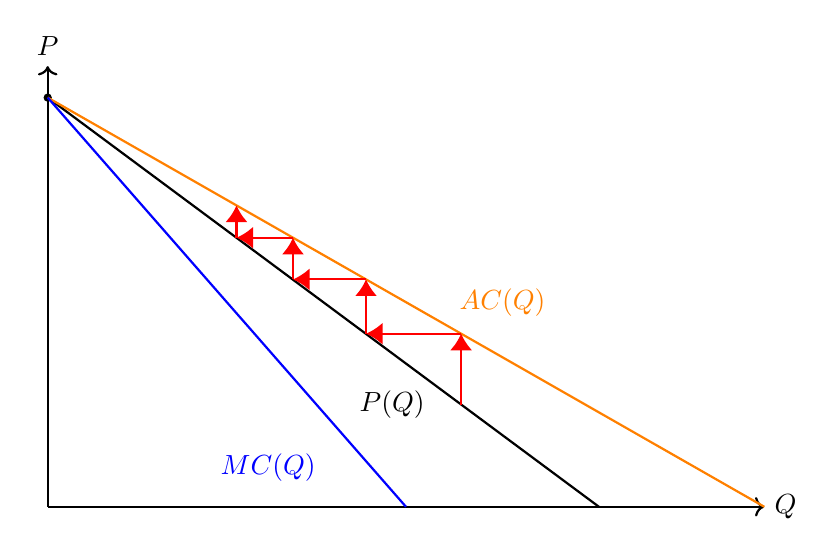
\begin{tikzpicture}[x=0.035cm, y=0.0020cm, scale=0.5]

    % Axes
    \draw[->, thick] (0,0) -- (520,0) node[right] {$Q$};
    \draw[->, thick] (0,0) -- (0,5600) node[above] {$P$};

    % Common intercept
    \fill (0,5200) circle[radius=3pt];

    % Demand curve: P(Q) = 5200 - 13Q
    \draw[thick] (0,5200) -- (400,0);
    \node at (250,1300) {$P(Q)$};

    % Average cost curve above demand: AC(Q) = 5200 - 10Q
    \draw[orange, thick] (0,5200) -- (520,0);
    \node[orange] at (330,2600) {$AC(Q)$};

    % Marginal cost curve below demand: MC(Q) = 5200 - 20Q
    \draw[blue, thick] (0,5200) -- (260,0);
    \node[blue] at (160,500) {$MC(Q)$};

    % ---------- UNRAVELING STEPS (full arrow tips, 4 cycles) ----------

    % Start at Q = 300 on demand
    \draw[-{Latex[length=6pt,width=8pt]}, thick, red] (300,1300) -- (300,2200);

    % Left to demand
    \draw[-{Latex[length=6pt,width=8pt]}, thick, red] (300,2200) -- (231,2200);

    % Up to AC
    \draw[-{Latex[length=6pt,width=8pt]}, thick, red] (231,2200) -- (231,2890);

    % Left to demand
    \draw[-{Latex[length=6pt,width=8pt]}, thick, red] (231,2890) -- (178,2890);

    % Up to AC
    \draw[-{Latex[length=6pt,width=8pt]}, thick, red] (178,2890) -- (178,3420);

    % Left to demand  (NEW CYCLE)
    \draw[-{Latex[length=6pt,width=8pt]}, thick, red] (178,3420) -- (137,3420);

    % Up to AC  (NEW CYCLE)
    \draw[-{Latex[length=6pt,width=8pt]}, thick, red] (137,3420) -- (137,3830);

\end{tikzpicture}
\end{center}
\end{frame}
%---------------------------------------------------------------------
\begin{frame}{Adverse selection}

    \newbold{Adverse selection} in health insurance:
    individuals buying insurance have worse health and/or higher expected costs than the individuals who choose to remain uninsured.\\
    $\implies$ The cost and demand curves \newbold{depend on each other}: \textit{selection market}
    $\implies$ \textit{Adverse selection}: the cost curves \newbold{slope down}\\
    \vspace{5mm}

    Could we have \newbold{advantageous} selection in a selection market? \only<2>{\newbold{yes}}
\end{frame}
%---------------------------------------------------------------------
\begin{frame}{Advantageous selection}

\begin{center}
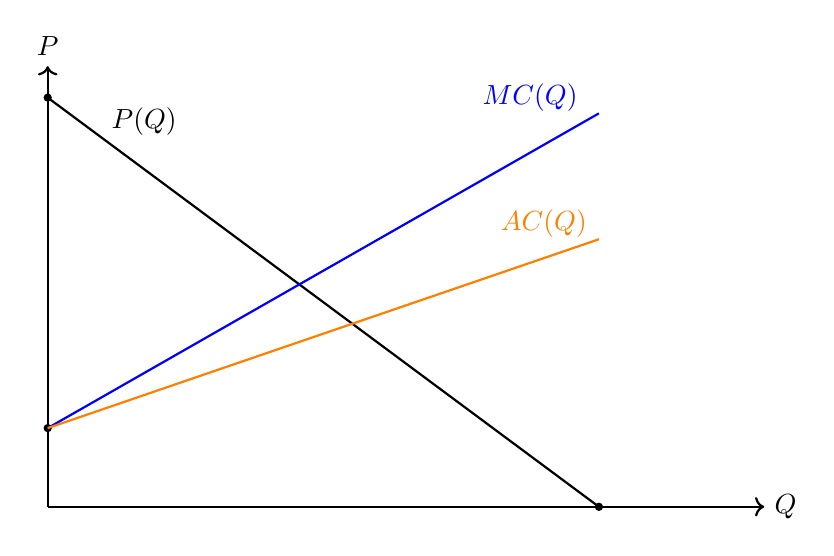
\begin{tikzpicture}[x=0.035cm, y=0.0020cm, scale=0.5]

    % Axes
    \draw[->, thick] (0,0) -- (520,0) node[right] {$Q$};
    \draw[->, thick] (0,0) -- (0,5600) node[above] {$P$};

    % Demand curve: P(Q) = 5200 - 13Q
    \draw[thick] (0,5200) -- (400,0);
    \node at (70,4900) {$P(Q)$};

    % Demand intercepts
    \fill (0,5200) circle[radius=3pt];
    \node[left] at (0,5200) {};

    \fill (400,0) circle[radius=3pt];
    \node[below] at (400,0) {};

    % Common low intercept for MC and AC
    \fill (0,1000) circle[radius=3pt];
    \node[left] at (0,1000) {};

    % Marginal cost: steeper increasing line
    % MC(Q) ≈ 1000 + 10Q
    \draw[blue, thick] (0,1000) -- (400,5000);
    \node[blue] at (350,5200) {$MC(Q)$};

    % Average cost: flatter increasing line
    % AC(Q) ≈ 1000 + 6Q
    \draw[orange, thick] (0,1000) -- (400,3400);
    \node[orange] at (360,3600) {$AC(Q)$};

\end{tikzpicture}
\end{center}

\end{frame}
%---------------------------------------------------------------------
\begin{frame}{Advantageous selection and overinsurance}

\begin{center}
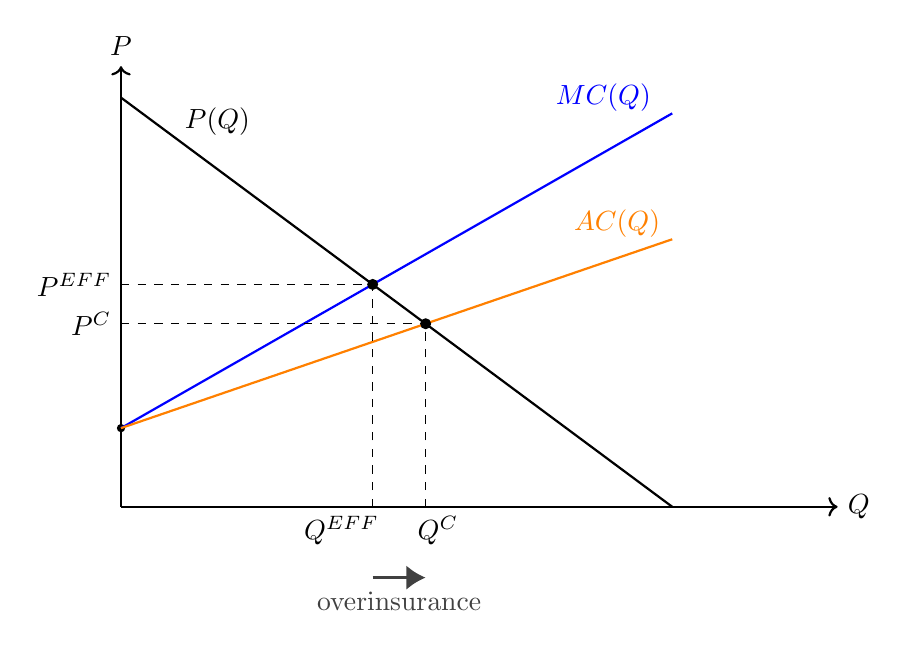
\begin{tikzpicture}[x=0.035cm, y=0.0020cm, scale=0.5]

    % Axes
    \draw[->, thick] (0,0) -- (520,0) node[right] {$Q$};
    \draw[->, thick] (0,0) -- (0,5600) node[above] {$P$};

    % Demand curve: P(Q) = 5200 - 13Q
    \draw[thick] (0,5200) -- (400,0);
    \node at (70,4900) {$P(Q)$};

    % Common low intercept for MC and AC
    \fill (0,1000) circle[radius=3pt];

    % Marginal cost: MC(Q) = 1000 + 10Q
    \draw[blue, thick] (0,1000) -- (400,5000);
    \node[blue] at (350,5200) {$MC(Q)$};

    % Average cost: AC(Q) = 1000 + 6Q
    \draw[orange, thick] (0,1000) -- (400,3400);
    \node[orange] at (360,3600) {$AC(Q)$};

    % ---------- Equilibria ----------

    % Efficient equilibrium: intersection of D and MC
    % Solve: 5200-13Q = 1000+10Q  => Q = 4200/23 ≈ 182.61, P ≈ 2826.09
    \fill (182.61,2826.09) circle[radius=4pt];
    \draw[dashed] (182.61,0) -- (182.61,2826.09);
    \draw[dashed] (0,2826.09) -- (182.61,2826.09);
    \node[below] at (160,0) {$Q^{EFF}$};
    \node[left]  at (0,2826.09) {$P^{EFF}$};

    % Perfect competition equilibrium: intersection of D and AC
    % Solve: 5200-13Q = 1000+6Q  => Q = 4200/19 ≈ 221.05, P ≈ 2326.32
    \fill (221.05,2326.32) circle[radius=4pt];
    \draw[dashed] (221.05,0) -- (221.05,2326.32);
    \draw[dashed] (0,2326.32) -- (221.05,2326.32);
    \node[below] at (230,0) {$Q^{C}$};
    \node[left]  at (0,2326.32) {$P^{C}$};

    % ---------- Over-insurance arrow under x-axis ----------
    % (requires \usetikzlibrary{arrows.meta} in the preamble)
    \draw[-{Latex[length=7pt,width=9pt]}, very thick, darkgray] (182.61,-900) -- (221.05,-900);
    \node[darkgray] at (201.8,-1200) {overinsurance};

\end{tikzpicture}
\end{center}

\end{frame}
%---------------------------------------------------------------------
\begin{frame}{Selection in health insurance}

    Selection:
    \begin{itemize}
        \item Adverse: cost curves slope down and the average cost is above the marginal cost\\
        $\implies$ Can result in underinsurance or completely unravel the market
        \item Advantageous: cost curves slope up and the average cost curve is below the marginal cost\\
        $\implies$ Can result in overinsurance
    \end{itemize}
    \vspace{5mm}

    This framework: graphical framework from \textit{Einav and Finkelstein (2011, Journal of Economic Perspectives)}\\
    \vspace{5mm}

    Which selection are you most worried about in health insurance?
\end{frame}
%---------------------------------------------------------------------
\begin{frame}{}
    \begin{center}
    \Large \textcolor{maroon}{Wrapping up}
    \end{center}
\end{frame}
%---------------------------------------------------------------------
\begin{frame}{What we covered today}
    \begin{itemize}
    \item Microeconomic review: perfect competition and monopolist
    \item Adverse selection {\footnotesize {\color{gray} (graphical framework from \textit{Einav and Finkelstein(2011, Journal of Economic Perspectives)})}}
    \begin{itemize}
        \item Selection markets
        \item Adverse selection and underinsurance
        \item Advantageous selection, unraveling
    \end{itemize}
\end{itemize}
\end{frame}
%---------------------------------------------------------------------
\begin{frame}{To next class}
\begin{itemize}
    \item \newbold{TO DO}
    \begin{enumerate}
        \item \newbold{Problem Set 3} has been posted: due \newbold{next Thursday 03/05 by 9:30am}
        \item Optional readings posted: \textit{Einav and Finkelstein (2011, JEP)} and \textit{Rothschild and Stiglitz (1976, QJE)}
        \item Review this class and past material $\implies$ \textit{questions on it?}
    \end{enumerate}
    \vspace{5mm}

    \item Program for next class
    \begin{itemize}
        \item Empirical evidence of adverse selection
        \item What does this framework teach us? Mandates and death spirals
    \end{itemize}
\end{itemize}
\end{frame}
%---------------------------------------------------------------------